\newcommand{\wf}{\mathrm{d}}
\newcommand{\e}{\mathrm{e}}
\newcommand{\curl}{\nabla\times}
\newcommand{\divi}{\nabla\cdot}

\chapter{虚位移简介}

\emph{编者注:本节作者为施杰亨。\\\\}

虚位移是分析力学的重要基本概念之一,
一般会在二秋学期的理论力学课程中系统学习,
为使行文不至于太长了(虽然已经很长了),
我们以下仅挑部分简单介绍,完整请参考《理论力学》。
(另外,也可以到赵爹书上看,但不推荐)

\section{约束}

大多数情况下,质点系的运动,除了外力影响外,
还会受内部的一些条件约束。\par
比如,一个单摆,摆锤的位置坐标需要满足\(x^2+y^2=l^2\),这是对位置的几何条件约束;
又如,纯滚条件\(\dot{\varphi} r=\dot{x}\),
这是与速度也有关的约束,称为运动约束,
当然这个条件可以通过积分变成只与位置有关的约束\(R\varphi=x\)。\par
一般的,我们可以把一个由\(n\)个质点组成的力学系统的约束条件表示为
\[f_l(\boldsymbol{r}_1,\boldsymbol{r}_2,
\dots,\boldsymbol{r}_n; \dot{\boldsymbol{r}}_1,
\dot{\boldsymbol{r}}_2,\dots,\dot{\boldsymbol{r}}_n;t)=0,
\quad l=1,2,3,\dots\]
\par
以下我们考虑理想约束,
可以把速度通过积分化为几何约束(可积分的运动约束和几何约束被称为完整约束),
即约束表达式中不含速度
\[f(\boldsymbol{r}_1,\boldsymbol{r}_2,\dots,\boldsymbol{r}_n;t)=0\]
\par
如果约束不直接依赖于时间,
其数学表达式不显含时间,
称为稳定约束;
如果约束明显依赖于时间,
其数学表达式显含时间,
称为不稳定约束。
比如前面提到的单摆即稳定约束。
但是如果我们把摆绳从固定点匀速释放,则约束条件化为
\(x^2+y^2-(l_0+vt)^2=0\),显含时间,是不稳定约束。
\par
当然我们还可以通过广义坐标来表示约束条件。
\[f(q_1,q_2,\dots,q_s;t)=0\]
另外,一个\(n\)自由度的系统,含\(m\)个理想约束,
则独立的广义坐标数为\(s=n-m\)。

\section{变分}

\subsection*{定义}
泛函:设\(C\)是函数(形式)的集合,\(B\)是实数的集合,
如果对\(C\)中每一个函数(形式)都有\(B\)中的实数与之对应,
则称\(F\)是\(q(t)\)的泛函,记为\(F[q(t)]\)。
可以认为泛函是函数的函数,\(q(t)\)是\(F[q(t)]\)的自变量。\par
泛函的变分:如果函数\(q(t)\)是泛函\(F[q(t)]\)定域内一任意函数,
如果\(q(t)\)变化为定域内另一新函数\(\bar{q}(t)\),
则\(\bar{q}(t)\)与\(q(t)\)的差\(\delta q(t)=\bar{q}(t)-q(t)\)是函数\(q(t)\)的变分。

区分以下概念:
\begin{itemize}
    \item 函数的值:取决于自变量的值和函数对应关系(函数形式) \(q(t)\)
    \item 函数的微分:自变量的值的微小改变量引起的函数值的改变量 \(\wf q=\dot{q}\wf t\)
    \item 函数的变分:同一\(t\)时,函数形式的微小改变引起的函数值的变化 \[\delta q(t)=\bar{q}(t)-q(t),\quad\quad\bar{q}(t)=q(t)+\delta q(t)\]
\end{itemize}

\subsection*{举例:}
\subsubsection*{1. \(q(t)=at^2,\,\bar{q}(t)=(a+\delta a)t^2\):}

\[\wf q=2at\wf t\]
\[\delta q=\bar{q}(t)-q(t)=\delta at^2\]

\subsubsection*{2. \(q(t)=t^a,\,\bar{q}(t)=t^{a+\delta a}\):}

\[\wf q=at^{a-1}\wf t\]
\[\delta q=\bar{q}(t)-q(t)=t^a\left(t^{\delta a}-1\right)\]
  
\section{虚位移}

\subsection*{定义}

质点在一个时间间隔\(\wf t\)内\textbf{实际}发生的位移,叫实位移。
用微分符号\(\wf\)表示,即
\[\wf\boldsymbol{r}=\wf x\hat{i}+\wf y\hat{j}+\wf z\hat{k}=\dot{\boldsymbol{r}}\wf t,\]
用广义坐标表示为
\[\wf\boldsymbol{r}=\sum\dfrac{\partial \boldsymbol{r}}{\partial q_i}\wf q_i+\dfrac{\partial \boldsymbol{r}}{\partial t}\wf t.\]

在某时刻\(t\),
在约束条件允许的情况下,
“想象”质点发生了一个极小的位移,就是虚位移,
用一个变分符号\(\delta\)表示。
注意:虚位移不是由时间变化引起的,
只取决于该时刻质点的位置和质点所受的约束条件。即:
\[\delta\boldsymbol{r}=\delta x\hat{i}+\delta y\hat{j}+\delta z\hat{k}, \quad (\delta t=0)\]
用广义坐标表示为
\[\delta\boldsymbol{r}=\sum\dfrac{\partial \boldsymbol{r}}{\partial q_i}\delta q_i.\]

下面考虑约束条件对实位移和虚位移的作用:

\subsubsection*{实位移}

\(\boldsymbol{r}\)和\(\boldsymbol{r}+\wf\boldsymbol{r}\)满足约束条件
\[\begin{cases}
    f(x,y,z,t)=0,\\
    f(x+\wf x,y+\wf y,z+\wf z,t+\wf t)=0
\end{cases}\]
作差
\[\dfrac{\partial f}{\partial x}\wf x+\dfrac{\partial f}{\partial y}\wf y+\dfrac{\partial f}{\partial z}\wf z+\dfrac{\partial f}{\partial t}\wf t=0\]
即
\[\wf f(\boldsymbol{r},t)=\nabla f\cdot\wf\boldsymbol{r}+\dfrac{\partial f}{\partial t}\wf t=0\]

\subsubsection*{虚位移}

\(\boldsymbol{r}\)和\(\boldsymbol{r}+\delta\boldsymbol{r}\)满足约束条件
\[\begin{cases}
    f(x,y,z,t)=0,\\
    f(x+\delta x,y+\delta y,z+\delta z,t)=0,\quad(\delta t=0)
\end{cases}\]
作差得到
\[\dfrac{\partial f}{\partial x}\delta x+\dfrac{\partial f}{\partial y}\delta y+\dfrac{\partial f}{\partial z}\delta z=0\]
即
\[\delta f(\boldsymbol{r},t)=\nabla f\cdot\delta\boldsymbol{r}=0\]
此即约束条件对虚位移的约束。

\subsection*{实位移和虚位移的关系}

实位移是由动力学方程决定的实际发生位移,是唯一确定的。
实位移连接运动轨迹上\(t\)和\(t+\wf t\)对应的两点,\(\wf\boldsymbol{r}\)沿运动轨迹的切向。
\par
虚位移则不需要满足动力学方程,可以有无穷多个。
虚位移连接两个可能的运动轨迹在某一时刻的对应点,
\(\delta \boldsymbol{r}\)使轨迹改变为\(\boldsymbol{r}+\delta\boldsymbol{r}\)。
虚位移需满足几何条件\(\nabla f\cdot\delta\boldsymbol{r}=0\)。
\par
简单地说,二者的区别是:实位移需满足运动方程,虚位移只需满足约束条件。
\par
对稳定约束,实位移是多个虚位移中的一个。
比如前面提到的单摆,
满足约束的虚位移沿圆周切向,有向左或向右两种可能;
而它的实位移还有该时刻的速度方向确定,只能是其中一个方向。
\par
对不稳定约束,实位移与虚位移不一定一致。
比如前面提到的摆绳变长的摆,
虚位移与普通单摆相同,但是实位移还有沿摆绳径向的分量。

\section{虚功原理的应用}

上课例题:如下图,有一根刚性长杆斜靠在墙角,长度为$2l$,与竖直方向的夹角为$\theta$,平衡时水平地面的摩擦力与弹力的比值为$\mu$,竖直墙面光滑。求平衡时的夹角$\theta$的值。

\begin{center}
    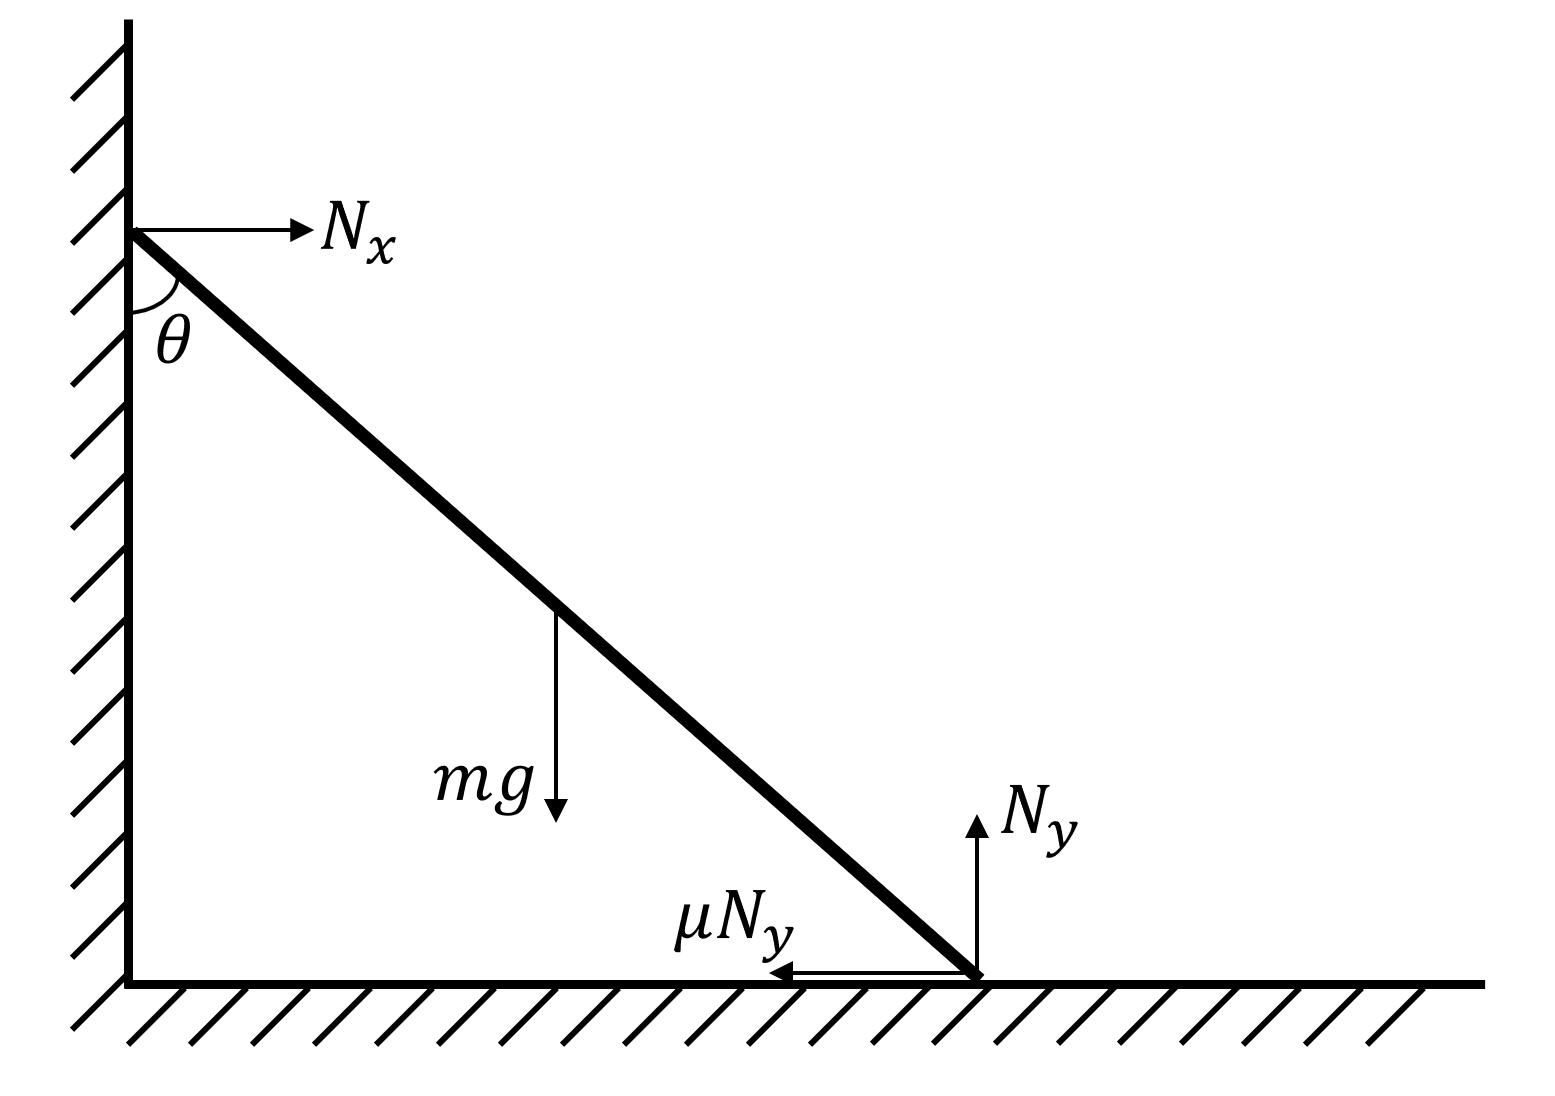
\includegraphics[height=120pt]{assets/Virtual_Displacement_Example.png}
\end{center}

容易发现系统只有一个自由度,
选取广义坐标\(\theta\),则
\[\begin{aligned}
    x_A&=2l\sin\theta,\\
    y_C&=l\cos\theta
\end{aligned}.\]

(此处在使用三角函数时,约束条件已经自动满足,如\(y_A=0,\,x_B=0\)。)

虚位移为
\begin{align*}
    \delta x_A&=2l\cos\theta\delta\theta,\\
    \delta y_C&=-l\sin\theta\delta\theta.
\end{align*}

平衡条件下各主动力总虚功为零
\[\delta W=0,\]
即
\[(-\mu N_Y)\delta x_A-Mg\delta y_C=0.\]

显然\(N_Y=Mg\)
\[(2\mu\cos\theta-\sin\theta)\delta\theta=0.\]
解得
\[\theta=\arctan2\mu.\]

\subsubsection*{}

本题只是虚功原理的简单应用,
我们并不能很好的感受到虚功原理对处理复杂问题的简化。
实际上,虚功原理的主要意义在于简化了约束反力对问题的影响。
我们可以从虚位移满足的条件中看到,约束反力在虚位移上不做功,
即虚功原理只需要处理主动力的做功,这大大简化了运算。
